% \pagebreak[4]
% \hspace*{1cm}
% \pagebreak[4]
% \hspace*{1cm}
% \pagebreak[4]
\newcommand\setrow[9]{
  \setcounter{col}{1}
  \foreach \n in {#1, #2, #3, #4, #5, #6, #7, #8, #9} {
    \edef\x{\value{col} - 0.5}
    \edef\y{9.5 - \value{row}}
    \node[anchor=center] at (\x, \y) {\n};
    \stepcounter{col}
  }
  \stepcounter{row}
}
\chapter{Recommender Systems}
\ifpdf
    \graphicspath{{Chapter1/Chapter1Figs/PN1G/}{Chapter1/Chapter1Figs/PDF/}{Chapter1/Chapter1Figs/}}
\else
    \graphicspath{{Chapter1/Chapter1Figs/EPS/}{Chapter1/Chapter1Figs/}}
\fi
\markright{\thechapter. Recommender System Basics}
\section{Basics}
To build an active sample selection algorithm, first a matrix completion one must be used. The basic idea such a system is graphically described in figure \ref{MatrixComp}. We have an incomplete matrix that tells us a certain amount of data about what movies each user likes or dislikes. From this we use a matrix completion algorithm to infer what the empty entries are. This thus allows a system to recommend potential movies a user may like or useful drug-target interactions that have not been tested out.
\begin{figure}[!htbp]
  \begin{center}
\begin{tikzpicture}[scale=.6]

  \begin{scope}
    \draw (0, 0) grid (9, 9);
    \draw[very thick, scale=9] (0, 0) grid (1, 1);

    \setcounter{row}{1}
    \setrow { }{3}{ }  {5}{ }{5}  { }{ }{ }
    \setrow {1}{ }{ }  { }{ }{ }  { }{4}{ }
    \setrow { }{ }{ }  {4}{3}{ }  {3}{ }{1}

    \setrow { }{3}{ }  { }{4}{ }  {1}{4}{ }
    \setrow { }{ }{2}  {4}{3}{ }  { }{4}{2}
    \setrow { }{ }{ }  { }{3}{ }  { }{ }{1}

    \setrow { }{1}{ }  {2}{ }{2}  { }{ }{ }
    \setrow { }{3}{ }  {4}{ }{ }  {1}{ }{2}
    \setrow { }{ }{ }  {4}{ }{ }  { }{4}{2}

	\node[anchor=center] at (4.5, 9.5) {Movies};
	\node[anchor=center, rotate=90] at (-0.5, 4.5) {Users};
    \node[anchor=center] at (4.5, -0.5) {Incomplete User-Movie Matrix};
  \end{scope}
  
   \begin{scope}
\tikzstyle{vecArrow} = [thick, decoration={markings,mark=at position
   1 with {\arrow[semithick]{open triangle 60}}},
   double distance=1.4pt, shorten >= 5pt,
   preaction = {decorate},
   postaction = {draw,line width=1.4pt, white,shorten >= 4.5pt}]
   
\draw [vecArrow](9.5,4.5) -- (11,4.5);

   \end{scope}

  \begin{scope}[xshift=12cm]
    \draw (0, 0) grid (9, 9);
    \draw[very thick, scale=9] (0, 0) grid (1, 1);

    \setcounter{row}{1}
    \setrow { }{3}{ }  {5}{ }{5}  { }{ }{ }
    \setrow {1}{ }{ }  { }{ }{ }  { }{4}{ }
    \setrow { }{ }{ }  {4}{3}{ }  {3}{ }{1}

    \setrow { }{3}{ }  { }{4}{ }  {1}{4}{ }
    \setrow { }{ }{2}  {4}{3}{ }  { }{4}{2}
    \setrow { }{ }{ }  { }{3}{ }  { }{ }{1}

    \setrow { }{1}{ }  {2}{ }{2}  { }{ }{ }
    \setrow { }{3}{ }  {4}{ }{ }  {1}{ }{2}
    \setrow { }{ }{ }  {4}{ }{ }  { }{4}{2}
    
	\node[anchor=center] at (4.5, 9.5) {Movies};
	\node[anchor=center, rotate=90] at (-0.5, 4.5) {Users};
    \node[anchor=center] at (4.5, -0.5) {Completed Matrix};

    \begin{scope}[blue, font=\sffamily\slshape]
      \setcounter{row}{1}
    \setrow {1}{ }{2}  { }{4}{ }  {2}{4}{2}
    \setrow { }{3}{2}  {4}{3}{4}  {1}{ }{2}
    \setrow {1}{2}{2}  { }{ }{4}  { }{3}{ }

    \setrow {1}{ }{2}  {4}{ }{4}  { }{ }{2}
    \setrow {1}{3}{ }  { }{ }{4}  {1}{ }{ }
    \setrow {1}{2}{1}  {3}{ }{3}  {1}{3}{ }

    \setrow {1}{ }{1}  { }{1}{ }  {1}{2}{1}
    \setrow {1}{ }{2}  { }{4}{4}  { }{4}{ }
    \setrow {1}{3}{2}  { }{3}{4}  {1}{ }{ }
    \end{scope}

  \end{scope}

\end{tikzpicture}
\end{center}
Completed entries have their number represented in blue. Each movie is rated out of 5.
    \caption{Sample Matrix Completion on Movie Data}
    \label{MatrixComp}
  
\end{figure}

Many commercial systems implementations of recommender systems currently exist. For example Amazon, YouTube, Google, Netflix, IMDb and Last.fm are but a small sample of websites using recommender systems to suggest films, ads, music or products to users. In fact Netflix is known for the "Netflix Prize", an open competition that awarded \$1 million to a group of researchers that could create a recommender system achieving a 10\% or more improvement on Netflix's own one.

More formally, a recommender system database comes in matrix form, $R \in \mathbb{R}^{M \times N}$ with each entry containing a numerical quantifier of the relationship between the row item and column item. As not every entry is complete we can associate this to a mask matrix $Z \in \mathbb{R}^{M \times N}$, where $Z_{ij} \in \{0,1\} \forall i,j$. $0$ represents an unknown entry and $1$ a currently known entry.


\nomenclature{RMSE}{Root Mean Square Error -  Measure of differences between values predicted by a model and the actual values:  $\sqrt{\frac{1}{N} \sum\nolimits_{i=1}^{N}(\hat{x}_i-x_i)^2}$}
\nomenclature{CF}{Collaborative Filtering} 
\nomenclature{PMF}{Probabilistic Matrix Factorisation} 
\nomenclature{BPMF}{Bayesian Probabilistic Matrix Factorisation} 



\section{Types of Recommender Systems}


\subsection{Overview}
Recommender systems typically work by having a pre-processing and analysis/matching stage with Figure \ref{fig:RecSysDiagram} showing the various stages. Pre-processing will typically be clustering the data into groups, reducing the dimensionality (for example by a process similar to SVD) or creating a subset of data that is more manageable. Active sample selection fits in here. Then the actual processing stage is where the empty samples are filled in. There can also be a post-processing stage where certain generated samples are selected either due to their usefulness or high score (i.e. a high predicted product score may be selected as part of a monetisation strategy). 

\nomenclature{SVD}{Singular Value Decomposition - A method to decompose a matrix into smaller dimension matrices}

There are several types of Recommender Systems:
\begin{description}[style=standard,leftmargin=.5cm,font=\bfseries]
\item[Collaborative Filtering] In this type of system the user is placed into sub-groups that have similar taste. From this, it is expected that if user A has similar taste than user B on some products he is more likely to have the same one about different products.
\item[Content-based filtering] In this system features are learned about content (such as item color, film type, music genre etc \ldots) and a user's profile of their tastes is built, allowing products to be recommended by their features rather than group similarity.
\item[Demographic Based] In this system extra data that groups columns or users into categories (based on age or sex for example) is used to recommend users items in their respective category.
\end{description}

Each of the above methods can be done in several different ways and have varying performance. It would thus make sense to select the Netflix prize winner algorithm. However the winning proposal, by a team named "BellKor's Pragmatic Chaos", consisted of an ensemble of various recommender systems. This increases complexity and is not very practical to work with. Thus an algorithm that performs well but simple (and easily built upon) is preferred. This explains the choice of the Probabilistic Matrix Factorisation algorithm. Its RMSE on the Netflix dataset is 0.8861, about 7\% better than Netflix system\footnote{The goal of the Netflix prize was to achieve a performance increase of 10\%}. Bayesian Probabilistic Matrix Factorisation \cite{SalMnih2008}, an extension of PMF, will also quickly be covered due to its good performance on very sparse datasets. Finally it decomposes a matrix into two feature matrices which turn out to be very useful in the goal of active sample selection.

\subsection{Probabilistic Matrix Factorisation}
\label{sec:pmf}
PMF works by assuming that each input sample comes with Gaussian noise. If we decompose $R$ into two matrices $\mathrm{U^{T} V}$ we can describe each item, with index $ij$ as $x_{ij}=\mathbf{u}_{i}^{T}\mathbf{v}_{j}+\epsilon_{ij}$ where $\epsilon_{ij} \sim  \mathcal{N} (0,\sigma^2_\epsilon)$. Equations \ref{eq:rsimeq} and \ref{eq:decomp} provide a quick intuition into the decomposition. The reason we decompose the matrix in two matrices is motivated by the want to extract features from each column and row item. This can be done by performing what is called a latent aspect model, which essentially creates a column and row matrices composed of the features and weightings of these items.
\begin{equation} \label{eq:rsimeq}
R \backsimeq U^{T} \cdot V
\end{equation}
\begin{equation}
 \label{eq:decomp}
U^{T} \cdot V=\begin{bmatrix}
u_{11} & u_{12} & \cdots \\
u_{21} & u_{22}& \cdots \\
u_{31}  & u_{32} & \cdots \\
u_{41}  & u_{42} & \cdots \\
\vdots  & \vdots & \ddots
\end{bmatrix} \cdot \begin{bmatrix}
v_{11} & v_{21} & v_{31} &  \cdots \\[-0.1em] 
v_{12} & v_{22} & v_{32} & \cdots \\[-0.1em]
\vdots & \vdots & \vdots &  \ddots \\[-0.1em]
\end{bmatrix}
\end{equation}

We can choose an arbitrary number of features $D$ to form the matrices $U \in \mathbb{R}^{D\times N}$ and $V \in \mathbb{R}^{D\times M}$. Essentially $U$ and $V$ contain the latent features of each row and column items, with $U_i$ and $V_j$ containing the row and column latent features. Assuming the Gaussian noise we can define the conditional distribution of $R$ as:
\begin{equation}
p(R|U,V,\sigma^2) = \prod_{i=1}^{N} \prod_{j=1}^{M} \left[\mathcal{N}(R_{ij}|U_i^T V_j,\sigma^2)\right]^{Z_{ij}}
\end{equation}
Remember that $Z$ is the mask matrix. $i$ and $j$ are the matrix entry coordinates. In addition to this we place Gaussian priors on row and column feature vectors:
\begin{eqnarray}
p(U|\sigma_U^2) = \prod_{i=1}^{N} \mathcal{N}(U_i|0,\sigma_U^2\mathbf{I}), &   p(V|\sigma_V^2) = \prod_{j=1}^{M} \mathcal{N}(V_j|0,\sigma_V^2\mathbf{I})
\end{eqnarray}
Now we assume row and column independence giving:
\begin{equation*}
P(U,V|\sigma_U^2\mathbf{I},\sigma_V^2\mathbf{I}) = p(U|\sigma_U^2)  p(V|\sigma_V^2)
\end{equation*}
We want to find the likelihood of $U$ and $V$ given the supplied parameters.
\begin{align*}
P(U,V|R,\sigma,\sigma_U^2\mathbf{I},\sigma_V^2\mathbf{I}) &= \dfrac{P(U,V,R|\sigma,\sigma_U^2\mathbf{I},\sigma_V^2\mathbf{I})}{P(R|\sigma^2)} \\
&= \dfrac{P(R|U,V,\sigma^2)P(U,V|\sigma_U^2\mathbf{I},\sigma_V^2\mathbf{I})}{P(R|\sigma^2)} \\
&= \dfrac{P(R|U,V,\sigma^2) p(U|\sigma_U^2)  p(V|\sigma_V^2)}{P(R|\sigma^2)}
\end{align*}
 We take the log likelihood of $P(U,V|R,\sigma,\sigma_U^2\mathbf{I},\sigma_V^2\mathbf{I})$ to maximise it.
\begin{align}
\ln (P(U,V|R,\sigma,\sigma_U^2\mathbf{I},\sigma_V^2\mathbf{I})) &= - \frac{1}{2 \sigma^2} \sum_{i=1}^{N} \sum_{j=1}^{M} Z_{ij}(R_{ij}-U_i^TV_j)^2 - \frac{1}{2\sigma_U^2} \sum_{i=1}^{N} \|U_i\|_{Fro}^2 
\notag \\ &  - \frac{1}{2\sigma_V^2} \sum_{j=1}^{M} \|V_j\|_{Fro}^2 + C \label{eq:pmf_ml_log}
\end{align}
Where C is a number not depending on $U$ or $V$. From this we can get an error function to minimise (by inverting the signs).

\begin{align}
E&=\sum_{i=1}^{N} \sum_{j=1}^{M} Z_{ij}(R_{ij}-U_i^TV_j)^2 + \frac{\lambda_U}{2}\sum_{i=1}^{N} \|U_i\|_{Fro}^2 
+ \frac{\lambda_V}{2} \sum_{j=1}^{M} \|V_j\|_{Fro}^2
\label{eq:pmf_err_func}
\end{align}

With $\lambda_U = \frac{\sigma^2}{\sigma_U^2}$ and $\lambda_V = \frac{\sigma^2}{\sigma_V^2}$ being regularisation parameters. We can remove the mask matrix from the equation and create a cell specific error function:
\begin{align*}
e_{ij}^2= (R_{ij}-U_i^TV_j)^2 + \frac{\lambda_U}{2}\sum_{i=1}^{N} \|U_i\|_{Fro}^2 
+ \frac{\lambda_V}{2} \sum_{j=1}^{M} \|V_j\|_{Fro}^2
\end{align*}

From $e_{ij}^2$ we can find $U$ $V$ satisfying $\underset{U,V}{\argmin} \, E$ through simple gradient descent \cite{nnmf-grad}. We use the simple but effective Widrow-Hoff learning rule:

\begin{align*}
U_{ik}^{t+1} &= U_{ik}^{t} - \mu \frac{\partial}{\partial U_{ik}}(e_{ij}^2) \\
&= U_{ik}^{t} + \mu (2 e_{ij}V_{jk} - \lambda_U  U_{ik}^{t})\\
V_{jk}^{t+1} &= V_{jk}^{t} - \mu \frac{\partial}{\partial V_{jk}}(e_{ij}^2) \\
&= V_{jk}^{t} + \mu (2 e_{ij}U_{ik} - \lambda_V  V_{jk}^{t})
\end{align*}
$k$ is the feature index, as defined by $D$, $\mu$ i{\tiny }s the learning rate and $t$ is the iteration index. The steps above are repeated until convergence (as defined by a custom criteria) or a fixed number of iterations. This allows us to learn the features of each column and row. Once $U$ and $V$ are learned we can estimate the full matrix by:
\begin{align}
\hat{R} = U^T V
\end{align}
For very large matrices where only a specific entry is needed a single entry can be predicted by $\hat{R}_{ij} = U_i^T V_j$.
\subsection{Bayesian Probabilistic Matrix Factorisation}
\label{sec:bpmf}
\begin{figure}[!ht]
  \begin{center}
    \begin{tabular}{cc}
      % model_pca.tex
%
% Copyright (C) 2012 Jaakko Luttinen
%
% This file may be distributed and/or modified
%
% 1. under the LaTeX Project Public License and/or
% 2. under the GNU General Public License.
%
% See the files LICENSE_LPPL and LICENSE_GPL for more details.

% PCA model

%\beginpgfgraphicnamed{model-pca}
\begin{tikzpicture}

  % Define nodes
  \node[obs]                               (y) {$R_{ij}$};
  \node[latent, above=of y, xshift=-1.5cm] (w) {$V_j$};
  \node[latent, above=of y, xshift=1.5cm]  (x) {$U_i$};
  \node[const, below=1.4cm of y]            (t) {$\alpha$};
  \node[const, above=1cm of w]            (av) {$\alpha_V$};
  \node[const, above=1cm of x]            (au) {$\alpha_U$};

  % Connect the nodes
  \edge {x,w,t} {y} ; %
  \edge {av}{w} ;
  \edge {au}{x} ;

  % Plates
  \plate {yx} {(x)(y)} {$i=1..N$} ;
  \plate {} {(w)(y)(yx.north west)(yx.south west)} {$j=1..M$} ;

\end{tikzpicture}
%\endpgfgraphicnamed

%%% Local Variables: 
%%% mode: tex-pdf
%%% TeX-master: "example"
%%% End: 
 &
      % model_pca.tex
%
% Copyright (C) 2012 Jaakko Luttinen
%
% This file may be distributed and/or modified
%
% 1. under the LaTeX Project Public License and/or
% 2. under the GNU General Public License.
%
% See the files LICENSE_LPPL and LICENSE_GPL for more details.

% PCA model

%\beginpgfgraphicnamed{model-pca}
\begin{tikzpicture}

  % Define nodes
  \node[obs]                               (y) {$R_{ij}$};
  \node[latent, above=of y, xshift=-1.5cm] (w) {$V_j$};
  \node[latent, above=of y, xshift=1.5cm]  (x) {$U_i$};
  \node[const, below=1.4cm of y]            (t) {$\alpha$};
  \node[latent, left=1cm of w]            (mv) {$\mu_V$};
  \node[latent, above=1cm of mv]            (lv) {$\Lambda_V$};
  \node[const, left=1cm of mv]            (m0v) {$\mu_0$};
  \node[const, above=1cm of lv]            (l0v) {$\nu_0$, $W_0$};
  
  \node[latent, right=1cm of x]            (mu) {$\mu_U$};
  \node[latent, above=1cm of mu]            (lu) {$\Lambda_U$};
  \node[const, right=1cm of mu]            (m0u) {$\mu_0$};
  \node[const, above=1cm of lu]            (l0u) {$\nu_0$, $W_0$};

  % Connect the nodes
  \edge {x,w,t} {y} ; %
  \edge {mv}{w} ;
  \edge {lv}{mv,w} ;
  \edge {m0v}{mv} ;
  \edge {l0v}{lv} ;
 
  \edge {mu}{x} ;
  \edge {lu}{mu,x} ;
  \edge {m0u}{mu} ;
  \edge {l0u}{lu} ;

  % Plates
  \plate {yx} {(x)(y)} {$i=1..N$} ;
  \plate {} {(w)(y)(yx.north west)(yx.south west)} {$j=1..M$} ;

\end{tikzpicture}
%\endpgfgraphicnamed

%%% Local Variables: 
%%% mode: tex-pdf
%%% TeX-master: "example"
%%% End: 
 \\
      PMF & BPMF
    \end{tabular}
  \end{center}
  \caption{Graphical Model for PMF and BPMF}
  \label{fig:bpmf_pmf_gm}
\end{figure}


Bayesian Probabilistic Matrix Factorisation has been proposed as an extension of PMF \cite{SalMnih2008}. It places Gaussian priors on $U$ and $V$ and Gaussian-Wishart priors on the row and column hyperparameters. A graphical representation to compare to PMF is found in figure \ref{fig:bpmf_pmf_gm}.

\begin{align*}
p(U|\mu_U,\Lambda_U) &= \prod\limits_{i=1}^{N} \mathcal{N}(U_i|\mu_U,\Lambda_U^{-1})\\
p(V|\mu_V,\Lambda_V) &= \prod\limits_{j=1}^{M} \mathcal{N}(V_j|\mu_V,\Lambda_V^{-1})
\end{align*}
$\Lambda^{-1}$ is the precision matrix and $\mu$ is the mean of each feature vector. $\Theta_U=\{\mu_U,\Lambda_U\}$ and $\Theta_V=\{\mu_V,\Lambda_V\}$ are defined as the row and column hyper parameters.
\begin{align*}
p(\Theta_U|\Theta_0) = p(\mu_U|\Lambda_U)p(\Lambda_U)= \mathcal{N}(\mu_U|\mu_0,(\beta_0 \Lambda_U)^{-1})\mathcal{W}(\Lambda_U|W_0, \nu_0) \\
p(\Theta_V|\Theta_0) = p(\mu_V|\Lambda_V)p(\Lambda_V)= \mathcal{N}(\mu_V|\mu_0,(\beta_0 \Lambda_V)^{-1})\mathcal{W}(\Lambda_V|W_0, \nu_0)
\end{align*}
We have $\mathcal{W}$ as the Wishart distribution with $\nu_0$ degrees of freedom and $W_0 \in \mathbb{R}^{D \times D}$. $\Theta_0=\{\mu_0,\nu_0,\Lambda_0\}$ is defined with $\mu_0=0$, $\nu_0=D$ and $W_0=\mathbf{I}_{D\times D}$.
After rearranging we end up with:
\begin{align*}
P(U,V|R,\Theta_U,\Theta_V) =\int \int P(R | U,V) P(U,V | R,\Theta_U,\Theta_V) P(\Theta_U,\Theta_V | \Theta_0)d\Theta_U d\Theta_V
\end{align*}
The above equation cannot be resolved analytically and approximate methods must be used. Thus we resort to a MCMC method, Gibbs sampling. This allows us to generate multiple approximations of $U$ and $V$ feature matrices and then get a better approximation out of it.
\nomenclature{MCMC}{Markov chain Monte Carlo - A means of approximating a probability distribution}
The outline of Gibbs sampling for BPMF is as follows:
\begin{enumerate}
  \item Initialise $U^1$, $V^1$
  \item For $t=1\dots T$
	\begin{itemize}
	  \item Sample hyperparameters $\Theta_U$ and $\Theta_V$
	  \item For $i=1 \dots N$ sample row features in parallel:
	  \begin{align*}
	  U_i^{t+1} \sim p(U_i^t|R, V^t ,\Theta_U^t)
	  \end{align*}
	  \item For $j=1 \dots M$ sample column features in parallel:
	  \begin{align*}
	  V_j^{t+1} \sim p(V_j^t|R, U^t ,\Theta_V^t)
	  \end{align*}
	\end{itemize}
\end{enumerate}
More details on BPMF and can be found in the appendix section \ref{sec:app_bpmf}.

For the purpose of this project it is mainly useful to remember that BPMF performs well on very sparse matrices - in  part due to the MCMC sampling process which provides a good approximation of the true probability distribution of data points.

\subsection{Kernelized Probabilistic Matrix Factorization}
\nomenclature{KMPF}{Kernelized Probabilistic Matrix Factorisation} 
Another variant of PMF that was tested was KMPF \cite{kpmf}. The main ideas to take from it are that it functions like PMF but with the crucial difference that a latent Gaussian process prior is placed over all rows and columns on top of a latent vector on each row and column. This means that it captures side information through kernel matrices that contain the covariance information. The intended use of these kernels is to use separate graph data, such as the social connection between users. However in the case this data does not exist a certain correlation between columns and rows can be assumed, which still results in good performances.

Performance of KPMF is best on very sparse data due to its ability to \textit{smooth} out data from its assumption of inter-row and inter-column correlation. In fact KPMF can work very well on empty rows or columns by filling them in with the most likely values - something PMF and BPMF struggle with.  Once more data on the dataset is available KPMF's performance can even be worse than the traditional model due to forcing these correlations. In the context of active sample selection, where more cells become available over time, this could cause a problem in determining the usefulness of each new discovered cell.
\section{Evaluation and comments}
\subsection{Performance test}

To understand what may be best to use we test each type of algorithm on a dataset. This allows to see its advantages and weaknesses. For the first test we look at figure \ref{fig:5pcmat}.

\begin{figure}[!htbp]
  \begin{center}
    \resizebox{\textwidth}{!}{% This file was created by matlab2tikz v0.4.7 running on MATLAB 8.1.
% Copyright (c) 2008--2014, Nico Schlömer <nico.schloemer@gmail.com>
% All rights reserved.
% Minimal pgfplots version: 1.3
% 
% The latest updates can be retrieved from
%   http://www.mathworks.com/matlabcentral/fileexchange/22022-matlab2tikz
% where you can also make suggestions and rate matlab2tikz.
% 
\begin{tikzpicture}

\begin{axis}[%
width=2.5in,
height=2.5in,
axis on top,
scale only axis,
xmin=0.5,
xmax=50.5,
y dir=reverse,
ymin=0.5,
ymax=80.5,
name=plot2,
title={BPMF $\beta$=1.5 D=10 RMSE=1.4858}
]
\addplot [forget plot] graphics [xmin=0.5,xmax=50.5,ymin=0.5,ymax=80.5] {5pcmatrix-1.png};
\end{axis}

\begin{axis}[%
width=2.5in,
height=2.5in,
axis on top,
scale only axis,
xmin=0.5,
xmax=50.5,
y dir=reverse,
ymin=0.5,
ymax=80.5,
name=plot1,
at=(plot2.left of south west),
anchor=right of south east,
title={PMF $\lambda$=0.1 D=10 RMSE=1.9269}
]
\addplot [forget plot] graphics [xmin=0.5,xmax=50.5,ymin=0.5,ymax=80.5] {5pcmatrix-2.png};
\end{axis}

\begin{axis}[%
width=2.5in,
height=2.5in,
scale only axis,
xmin=0,
xmax=200,
xlabel={Iterations},
xmajorgrids,
ymin=0,
ymax=3,
ylabel={Training RMSE},
ymajorgrids,
name=plot4,
at=(plot1.below south west),
anchor=above north west,
title={PMF learning rate}
]
\addplot [color=blue,solid,forget plot]
  table[row sep=crcr]{1	2.9957906513364\\
2	2.99573240721177\\
3	2.99567087079752\\
4	2.99560398509265\\
5	2.99552944277968\\
6	2.99544457608174\\
7	2.99534622706284\\
8	2.99523059115264\\
9	2.99509302512218\\
10	2.99492780867601\\
11	2.99472784614834\\
12	2.99448429136208\\
13	2.99418607436785\\
14	2.99381930334373\\
15	2.99336650821599\\
16	2.99280568438519\\
17	2.99210908521507\\
18	2.99124170073898\\
19	2.99015934778069\\
20	2.98880628441992\\
21	2.98711225159157\\
22	2.98498884051027\\
23	2.98232509328052\\
24	2.97898227636352\\
25	2.97478783909222\\
26	2.96952870557859\\
27	2.9629442777942\\
28	2.95471988090916\\
29	2.94448187572308\\
30	2.93179626868344\\
31	2.91617324245813\\
32	2.89708032539367\\
33	2.87396644545731\\
34	2.84629732187906\\
35	2.81359927710866\\
36	2.77550428936809\\
37	2.73178610650202\\
38	2.68237855815169\\
39	2.62737436043846\\
40	2.56701265929176\\
41	2.50166889237266\\
42	2.43185545900871\\
43	2.35822904747324\\
44	2.2815908321882\\
45	2.20286717493098\\
46	2.12306850148217\\
47	2.04323341127009\\
48	1.96436780813024\\
49	1.88738658206482\\
50	1.813063007095\\
51	1.74199062760765\\
52	1.67456234235614\\
53	1.61096952933276\\
54	1.55122034782063\\
55	1.49517255046433\\
56	1.44257397351365\\
57	1.39310389892452\\
58	1.34641012611975\\
59	1.30213885061277\\
60	1.25995649081079\\
61	1.21956401494873\\
62	1.18070504334836\\
63	1.14316918830491\\
64	1.10679195620598\\
65	1.07145225951035\\
66	1.03706829752675\\
67	1.00359233383394\\
68	0.971004748523338\\
69	0.939307669076093\\
70	0.908518462325837\\
71	0.878663374149575\\
72	0.84977160838898\\
73	0.82187012422418\\
74	0.794979392714515\\
75	0.76911028767131\\
76	0.744262199288707\\
77	0.720422361470927\\
78	0.69756628832028\\
79	0.675659134456531\\
80	0.654657737871361\\
81	0.634513078513625\\
82	0.615172890885836\\
83	0.596584199641218\\
84	0.578695595085115\\
85	0.561459121046717\\
86	0.544831702289787\\
87	0.528776086465032\\
88	0.513261313526749\\
89	0.498262753077555\\
90	0.483761768507088\\
91	0.469745078018227\\
92	0.456203888584848\\
93	0.443132880925406\\
94	0.430529122417648\\
95	0.418390980711125\\
96	0.406717103562855\\
97	0.39550552013768\\
98	0.384752905992009\\
99	0.374454038929302\\
100	0.36460145699923\\
101	0.355185314470331\\
102	0.346193418011223\\
103	0.337611414716886\\
104	0.329423096750327\\
105	0.321610784462664\\
106	0.314155750631027\\
107	0.307038652236959\\
108	0.300239942077499\\
109	0.29374023946558\\
110	0.287520646425914\\
111	0.281563002403608\\
112	0.275850076089079\\
113	0.27036569727607\\
114	0.265094834664483\\
115	0.260023627300645\\
116	0.255139378109963\\
117	0.250430517955989\\
118	0.245886548091405\\
119	0.241497967960482\\
120	0.237256194240643\\
121	0.233153475901463\\
122	0.229182809001198\\
123	0.225337853988034\\
124	0.221612857453017\\
125	0.218002579602373\\
126	0.214502228173589\\
127	0.211107399099781\\
128	0.207814023914021\\
129	0.204618323661903\\
130	0.201516768939631\\
131	0.198506045580991\\
132	0.195583025466306\\
133	0.192744741908713\\
134	0.189988369078752\\
135	0.18731120495017\\
136	0.184710657282246\\
137	0.182184232192865\\
138	0.179729524918503\\
139	0.177344212400268\\
140	0.175026047377274\\
141	0.172772853708979\\
142	0.170582522685899\\
143	0.168453010122892\\
144	0.166382334060845\\
145	0.164368572930905\\
146	0.162409864060639\\
147	0.160504402423542\\
148	0.158650439552621\\
149	0.156846282555277\\
150	0.155090293180899\\
151	0.153380886904451\\
152	0.151716531999314\\
153	0.150095748580831\\
154	0.148517107608674\\
155	0.146979229841494\\
156	0.145480784741487\\
157	0.144020489329753\\
158	0.142597106995693\\
159	0.14120944626541\\
160	0.13985635953521\\
161	0.138536741777016\\
162	0.137249529222785\\
163	0.135993698035103\\
164	0.134768262970903\\
165	0.133572276044958\\
166	0.132404825199296\\
167	0.131265032984191\\
168	0.130152055255781\\
169	0.129065079894787\\
170	0.128003325550198\\
171	0.126966040411223\\
172	0.12595250101023\\
173	0.12496201105892\\
174	0.123993900319442\\
175	0.123047523511773\\
176	0.122122259258242\\
177	0.121217509065769\\
178	0.120332696346031\\
179	0.119467265473537\\
180	0.118620680881329\\
181	0.117792426193838\\
182	0.116982003396267\\
183	0.116188932039702\\
184	0.115412748481079\\
185	0.11465300515702\\
186	0.113909269890489\\
187	0.113181125229173\\
188	0.112468167814452\\
189	0.111770007779813\\
190	0.11108626817754\\
191	0.110416584432518\\
192	0.109760603822016\\
193	0.109117984980294\\
194	0.108488397426935\\
195	0.107871521117811\\
196	0.107267046017633\\
197	0.10667467169305\\
198	0.106094106925321\\
199	0.105525069341596\\
200	0.104967285063899\\
};
\end{axis}

\begin{axis}[%
width=2.5in,
height=2.5in,
axis on top,
scale only axis,
xmin=0.5,
xmax=50.5,
y dir=reverse,
ymin=0.5,
ymax=80.5,
name=plot5,
at=(plot4.right of south east),
anchor=left of south west,
title={Original Data}
]
\addplot [forget plot] graphics [xmin=0.5,xmax=50.5,ymin=0.5,ymax=80.5] {5pcmatrix-3.png};
\end{axis}

\begin{axis}[%
width=2.5in,
height=2.5in,
axis on top,
scale only axis,
xmin=0.5,
xmax=50.5,
y dir=reverse,
ymin=0.5,
ymax=80.5,
name=plot6,
at=(plot5.right of south east),
anchor=left of south west,
title={Data available to algorithms 5\%}
]
\addplot [forget plot] graphics [xmin=0.5,xmax=50.5,ymin=0.5,ymax=80.5] {5pcmatrix-4.png};
\end{axis}

\begin{axis}[%
width=2.5in,
height=2.5in,
axis on top,
scale only axis,
xmin=0.5,
xmax=50.5,
y dir=reverse,
ymin=0.5,
ymax=80.5,
at=(plot6.above north west),
anchor=below south west,
title={KPMF $\sigma$=8 D=10 RMSE=1.3254}
]
\addplot [forget plot] graphics [xmin=0.5,xmax=50.5,ymin=0.5,ymax=80.5] {5pcmatrix-5.png};
\end{axis}
\end{tikzpicture}%}
    Each colour is made to represent a rating out of 5. Dark blue represents a 1 and red a rating of 5. The mean is represented in green.
    
    A row could be used to represent a user and a column a movie.
    \caption{Rating Predictions on synthetic data 5\% complete}
     \label{fig:5pcmat}
  \end{center}
\end{figure}
\begin{figure}[!htbp]
  \begin{center} 
    \resizebox{\textwidth}{!}{% This file was created by matlab2tikz v0.4.7 running on MATLAB 8.1.
% Copyright (c) 2008--2014, Nico Schlömer <nico.schloemer@gmail.com>
% All rights reserved.
% Minimal pgfplots version: 1.3
% 
% The latest updates can be retrieved from
%   http://www.mathworks.com/matlabcentral/fileexchange/22022-matlab2tikz
% where you can also make suggestions and rate matlab2tikz.
% 
\begin{tikzpicture}

\begin{axis}[%
width=2.5in,
height=2.5in,
axis on top,
scale only axis,
xmin=0.5,
xmax=50.5,
y dir=reverse,
ymin=0.5,
ymax=80.5,
name=plot2,
title={BPMF $\beta$=4 D=7 RMSE=1.0815}
]
\addplot [forget plot] graphics [xmin=0.5,xmax=50.5,ymin=0.5,ymax=80.5] {15pcmatrix-1.png};
\end{axis}

\begin{axis}[%
width=2.5in,
height=2.5in,
axis on top,
scale only axis,
xmin=0.5,
xmax=50.5,
y dir=reverse,
ymin=0.5,
ymax=80.5,
at=(plot2.left of south west),
anchor=right of south east,
title={PMF $\lambda$=0.01 D=7 RMSE=1.1015}
]
\addplot [forget plot] graphics [xmin=0.5,xmax=50.5,ymin=0.5,ymax=80.5] {15pcmatrix-2.png};
\end{axis}

\begin{axis}[%
width=2.5in,
height=2.5in,
axis on top,
scale only axis,
xmin=0.5,
xmax=50.5,
y dir=reverse,
ymin=0.5,
ymax=80.5,
at=(plot2.right of south east),
anchor=left of south west,
title={Data available to algorithms 15\%}
]
\addplot [forget plot] graphics [xmin=0.5,xmax=50.5,ymin=0.5,ymax=80.5] {15pcmatrix-3.png};
\end{axis}
\end{tikzpicture}%}
    For KPMF: RMSE=1.1867 for $\sigma=10$
    \caption{Rating Predictions on synthetic data 15\% complete}
    \label{fig:15pcmat}
  \end{center}
\end{figure}
For this figure data was randomly generate by generating 2 matrices $U \in \mathbb{R}^{80\times 5}$ and $V \in \mathbb{R}^{50\times 5}$, that is 5 latent features. A  random mask allowing the variants of PMF to only access 5\% of the data was made and used for matrix completion. The Root Mean Square Error(RMSE) of the predicted data was used as a measure of success. According to RMSE the best performing algorithm is KPMF, which was on average 1.3 off the real value. However all it has effectively done is predicted the mean with some amount of variation for all unknown values. We can see the effect of Gibbs sampling from BPMF as it captures the data distribution better than PMF or KPMF. Despite this it has a higher RMSE. This is one weakness of RMSE as some data sets may penalise more for guessing a value off the mean than one nearer to the mean. Finally PMF is seen to perform the worse, simply failing to predict many entries having very little information.

Making more data available, such as 15 \% of the dataset lead to an improvement for both BPMF and PMF as seen in figure \ref{fig:15pcmat}. PMF experienced the largest RMSE decrease -  something to keep in mind for sample selection. KPMF's RMSE has also improved however its output did not look any better.
\begin{figure}[!htbp]
  \begin{center}
    \resizebox{\textwidth}{!}{% This file was created by matlab2tikz v0.4.7 running on MATLAB 8.1.
% Copyright (c) 2008--2014, Nico Schlömer <nico.schloemer@gmail.com>
% All rights reserved.
% Minimal pgfplots version: 1.3
% 
% The latest updates can be retrieved from
%   http://www.mathworks.com/matlabcentral/fileexchange/22022-matlab2tikz
% where you can also make suggestions and rate matlab2tikz.
% 
\begin{tikzpicture}

\begin{axis}[%
width=2.5in,
height=2.5in,
axis on top,
scale only axis,
xmin=0.5,
xmax=300.5,
y dir=reverse,
ymin=0.5,
ymax=300.5,
name=plot2,
title={BPMF $\beta$=3.5 D=120 RMSE=0.4224}
]
\addplot [forget plot] graphics [xmin=0.5,xmax=300.5,ymin=0.5,ymax=300.5] {eiffel_tower-1.png};
\end{axis}

\begin{axis}[%
width=2.5in,
height=2.5in,
axis on top,
scale only axis,
xmin=0.5,
xmax=300.5,
y dir=reverse,
ymin=0.5,
ymax=300.5,
name=plot1,
at=(plot2.left of south west),
anchor=right of south east,
title={PMF $\lambda$=0.01 D=120 RMSE=0.36275}
]
\addplot [forget plot] graphics [xmin=0.5,xmax=300.5,ymin=0.5,ymax=300.5] {eiffel_tower-2.png};
\end{axis}

\begin{axis}[%
width=2.5in,
height=2.5in,
axis on top,
scale only axis,
xmin=0.5,
xmax=300.5,
y dir=reverse,
ymin=0.5,
ymax=300.5,
name=plot4,
at=(plot1.below south west),
anchor=above north west,
title={PMF $\lambda$=0.05 D=150 RMSE=0.3666}
]
\addplot [forget plot] graphics [xmin=0.5,xmax=300.5,ymin=0.5,ymax=300.5] {eiffel_tower-3.png};
\end{axis}

\begin{axis}[%
width=2.5in,
height=2.5in,
axis on top,
scale only axis,
xmin=0.5,
xmax=300.5,
y dir=reverse,
ymin=0.5,
ymax=300.5,
name=plot5,
at=(plot4.right of south east),
anchor=left of south west,
title={Original Image}
]
\addplot [forget plot] graphics [xmin=0.5,xmax=300.5,ymin=0.5,ymax=300.5] {eiffel_tower-4.png};
\end{axis}

\begin{axis}[%
width=2.5in,
height=2.5in,
axis on top,
scale only axis,
xmin=0.5,
xmax=300.5,
y dir=reverse,
ymin=0.5,
ymax=300.5,
name=plot6,
at=(plot5.right of south east),
anchor=left of south west,
title={Data available to algorithms 88.23\%}
]
\addplot [forget plot] graphics [xmin=0.5,xmax=300.5,ymin=0.5,ymax=300.5] {eiffel_tower-5.png};
\end{axis}

\begin{axis}[%
width=2.5in,
height=2.5in,
axis on top,
scale only axis,
xmin=0.5,
xmax=300.5,
y dir=reverse,
ymin=0.5,
ymax=300.5,
at=(plot6.above north west),
anchor=below south west,
title={KPMF $\sigma$=10 D=120 RMSE=0.6856}
]
\addplot [forget plot] graphics [xmin=0.5,xmax=300.5,ymin=0.5,ymax=300.5] {eiffel_tower-6.png};
\end{axis}
\end{tikzpicture}%}
    Image corrupted by drawing over and virtual spray paint
    \caption{Image Restoration}
    \label{fig:eiffel_tower}
  \end{center}
\end{figure}

In an effort to better understand each algorithm an image restoration trial was done. This is possible due to the rows and columns (pixel wise) in images to exhibit features about them. For example a column may have features indicating 45\% sky hue, 25\% Eiffel tower hue and 30\% ground hue with a row another having its own distribution. Multiplying both together would give the best estimate of the pixel at the specific row-column combination.
In figure \ref{fig:eiffel_tower} a picture with drawing over was supplied to each PMF variant. This was equivalent with supplying 88\% of the data. This time the scales are reversed, with PMF coming out as the clear winner. Not only is the image very similar to the original but little corruption in the overall restoration happened. BPMF failed at this task and distorted the picture overall, blurring it up\footnote{In a practical application of this algorithm it would be possible to only replace the unknown pixels.}. KPMF was able to restore the know pixels correctly but did not do a good job of predicting the missing ones, choosing to predict the mean color instead. KMPF is supposed to provide superior image restoration if supplied the correct kernel \cite{kpmf}. However, despite providing a diffusion kernel indicating that each pixel is correlated to its neighbouring ones, KPMF did not live up to the task.


For the purpose of this project mainly PMF and BPMF will be used as they showed the most promising performances and can be easily customised and built upon. This is especially useful as active sampling builds on top of recommender systems.

Note that the used datasets, synthetic and movielens, have their values ranging from 1 to 5. Thus a RMSE of 2 would mean that predictions are off by 2 stars on average. A good RMSE would thus be under 1, meaning movie predictions are only off by 1 star or less. When possible, other datasets used will be normalised between 1 and 5 to have the RMSE somewhat comparable.

\subsection{Choosing parameters}
All the above PMF variants all relied on one or many parameters. For example PMF uses\footnote{This is actually a combination of $\lambda_U$ and $\lambda_V$ from equation \ref{eq:pmf_err_func}} $\lambda$. These parameters nearly always affect the system performance and choosing them correctly is essential. While it is possible optimise them as such:
\begin{align*}
\underset{U,V,\lambda}{\argmin}\, E(U,V,\lambda)
\end{align*}
This is not a good idea. Indeed $\lambda$ is a regularisation parameter needed to allow the function to correctly generalise\footnote{In an optimisation context it can be seen as a Lagrange multiplier that enforces a constraint} and if optimised in a similar way it would tend to 0 defeating its purpose, see \ref{sec:lag_lambd_optim}. It would essentially perfectly (over)fit the data but not perform predictions correctly. 

Other parameters, such as D (the number of features), could be optimised in a similar way but this increases complexity necessarily. Instead these parameters are usually tweaked by hand and this is what has been done here as this is not the main focus of research.
\subsubsection{Learning rate $\mu$}

$\mu$ is an essential parameter to most iterative learning algorithms. It is appropriately called the learning rate as it defines the rate at which parameters are learnt. If we imagine a convex curve and we are located at a random location on it $\mu$ essentially defines how far we can go on each iteration to get closer to the minimum. Should it be too small a very high number of iterations will be needed to reach satisfactory performance. A too large learning rate may fail to converge due to the steps "jumping around" a minimum but never reaching it - alternatively it could simply overflow with the error increasing at each iteration.

\subsection{Pre-Processing datasets}
Before processing data, it is often advisable to pre-process it. This means cleaning up the data in ways that ensure good performance.
\subsubsection{Normalisation}
The first step that is often taken is to normalise data between two values - by convention 0 and 1 \footnote{For other types of learning algorithms normalisation may be between $[-1,1]$ and zero meaned.}. This ensures that some parameters used, such as regularisation or precision, need not be tweaked a lot when switching between datasets. Additionally when performing gradient descent (as in section \ref{sec:pmf}) over multiple dimensions it is preferable the error for each datapoint is in a similar order of magnitude.
\subsubsection{Discrete Data}
Discrete data is data that only takes a fixed number of values, which is applicable to movie-user datasets where a 5 star rating is given. To process these data is first be normalised between 0 and 1, 0 representing 1 and 1 representing 5. From this, parameters are learnt and data can be predicted. Placing the values back between 1 and 5 will result in non-integer values. Expectedly values are rounded up or down accordingly. Since $3.1$ and $3.45$ will both be rounded down to $3$ we can use the decimal as a measure of uncertainty, that is $3.1$ has a greater probability of actually being $3$ rather than $3.45$. While this is not a fail safe system the deviation from the discrete values can be useful for measuring uncertainty in the model.
\subsection{Online vs Offline learning}
Usually data will be fed to an algorithm and parameters returned to be used for prediction. However there are instances when new data points will be made available and a better performance will be achieved by retraining the parameters with the new data. When a model is retrained from scratch it is said to be done offline. Doing it online means training it once initially and then only carrying out a few steps to update the model when a new sample is received. Collaborative Filtering Algorithms, such as PMF, can be made online \cite{onlinepmf} by first training $U$ and $V$ for initial data and then updating these parameters at each incoming sample.

\begin{table}[!htb]
 \begin{tabular}{l|p{0.4\textwidth}|p{0.4\textwidth}|}
  & \textbf{Online} & \textbf{Offline} \\ \hline
  \textbf{Pro} & Fast update, less iterations  &  Adapts better to new items \\
 & Reuses parameters  & Less local minima issues   \\  \hline
    \textbf{Con} &   Can get stuck in local minima  &     Time intensive    \\
    & & Reinitialises parameters \\
    \hline
 \end{tabular}
 \caption{Comparison of online and offline matrix completion algorithms}
 \label{table:online_offline}
\end{table}


Table \ref{table:online_offline} shows a comparison of the pros and cons of online and offline learning for matrix factorisation systems. The general problem with online PMF is that the error function for PMF \ref{eq:pmf_err_func} is biconvex in $U$ and $V$ and that the minimum is found by alternatively updating each variable, which does not ensure global minimum. Thus if the parameters are stuck in a local minimum online updating will not help and randomly reinitialising them will be better. This is why we will default to using offline updating for the purpose of this report.


\subsection{Test and Validation dataset}
\begin{figure}[!htbp]
  \begin{center} 
    \resizebox{\textwidth}{!}{% This file was created by matlab2tikz v0.4.7 running on MATLAB 8.1.
% Copyright (c) 2008--2014, Nico Schlömer <nico.schloemer@gmail.com>
% All rights reserved.
% Minimal pgfplots version: 1.3
% 
% The latest updates can be retrieved from
%   http://www.mathworks.com/matlabcentral/fileexchange/22022-matlab2tikz
% where you can also make suggestions and rate matlab2tikz.
% 
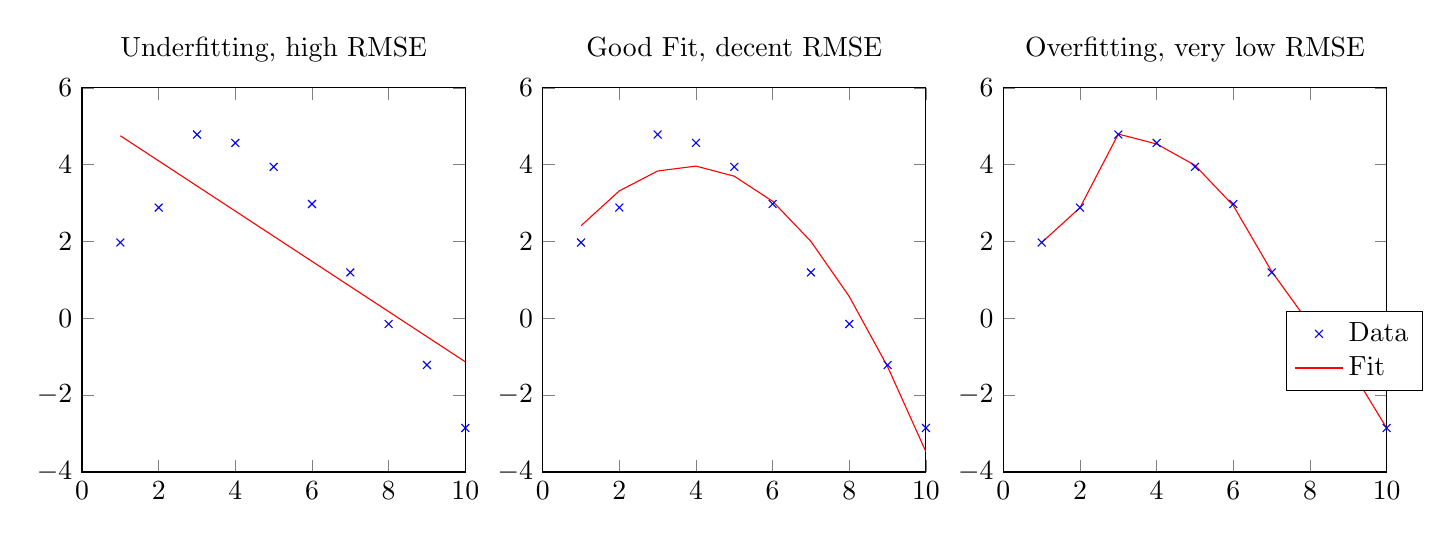
\begin{tikzpicture}

\begin{axis}[%
width=1.91620621980676in,
height=1.92052083333333in,
scale only axis,
xmin=0,
xmax=10,
ymin=-4,
ymax=6,
name=plot2,
title={Good Fit, decent RMSE}
]
\addplot [color=blue,only marks,mark=x,mark options={solid},forget plot]
  table[row sep=crcr]{1	1.97374569656748\\
2	2.88406786873516\\
3	4.78553661488987\\
4	4.5675745314657\\
5	3.94342674696089\\
6	2.9770548882854\\
7	1.19483170610871\\
8	-0.14695915605463\\
9	-1.21420046517419\\
10	-2.85419171271952\\
};
\addplot [color=red,solid,forget plot]
  table[row sep=crcr]{1	2.41023287753905\\
2	3.31851727633452\\
3	3.83626634177898\\
4	3.96348007387242\\
5	3.70015847261484\\
6	3.04630153800625\\
7	2.00190927004665\\
8	0.566981668736026\\
9	-1.25848126592561\\
10	-3.47447953393826\\
};
\end{axis}

\begin{axis}[%
width=1.91620621980676in,
height=1.92052083333333in,
scale only axis,
xmin=0,
xmax=10,
ymin=-4,
ymax=6,
at=(plot2.left of south west),
anchor=right of south east,
title={Underfitting, high RMSE}
]
\addplot [color=blue,only marks,mark=x,mark options={solid},forget plot]
  table[row sep=crcr]{1	1.97374569656748\\
2	2.88406786873516\\
3	4.78553661488987\\
4	4.5675745314657\\
5	3.94342674696089\\
6	2.9770548882854\\
7	1.19483170610871\\
8	-0.14695915605463\\
9	-1.21420046517419\\
10	-2.85419171271952\\
};
\addplot [color=red,solid,forget plot]
  table[row sep=crcr]{1	4.75344487764515\\
2	4.09958794303656\\
3	3.44573100842797\\
4	2.79187407381938\\
5	2.13801713921079\\
6	1.48416020460219\\
7	0.830303269993603\\
8	0.176446335385012\\
9	-0.47741059922358\\
10	-1.13126753383217\\
};
\end{axis}

\begin{axis}[%
width=1.91620621980676in,
height=1.92052083333333in,
scale only axis,
xmin=0,
xmax=10,
ymin=-4,
ymax=6,
at=(plot2.right of south east),
anchor=left of south west,
title={Overfitting, very low RMSE},
legend style={at={(0.737312217300616,0.210441045204993)},anchor=south west,draw=black,fill=white,legend cell align=left}
]
\addplot [color=blue,only marks,mark=x,mark options={solid}]
  table[row sep=crcr]{1	1.97374569656748\\
2	2.88406786873516\\
3	4.78553661488987\\
4	4.5675745314657\\
5	3.94342674696089\\
6	2.9770548882854\\
7	1.19483170610871\\
8	-0.14695915605463\\
9	-1.21420046517419\\
10	-2.85419171271952\\
};
\addlegendentry{Data};

\addplot [color=red,solid]
  table[row sep=crcr]{1	1.97407548210884\\
2	2.88109979888774\\
3	4.79740889434664\\
4	4.53987254606422\\
5	3.98497972506559\\
6	2.93550191018698\\
7	1.22253369151728\\
8	-0.158831435498733\\
9	-1.21123239530863\\
10	-2.85452149827793\\
};
\addlegendentry{Fit};

\end{axis}
\end{tikzpicture}%}
    \caption{Examples of different model fitting}
    \label{fig:over_underfit}
  \end{center}
\end{figure}
From section \ref{sec:pmf} we see that learning from a dataset involves minimising an error function. The problem with this is that we are subject to a "tunnel vision" where only the given data is considered while minimising the error function. A model that only fits the test data, as in figure \ref{fig:over_underfit}, can overfit it and not generalise well. This is one of the reason the regularisation parameters $\lambda_U$ and $\lambda_V$ exist, as they avoid $U$ and $V$ becoming too large and only being specific to the test data. Another way to avoid this is to consider splitting up the dataset into a test set and a validation set. The test set will be used for training. However at each parameter step update, we can calculate the RMSE from the validation data - i.e. data not used for training. As soon as a step is found to lead to an increase of validation RMSE we can infer that the model is potentially starting to overfit and stopping training of parameters is preferable.

\subsection{Data quality}
Another issue with any machine learning system is that of data quality. Any inaccurate or badly generated data can prove to be a major bottleneck in the performance of machine learning systems. Many datasets, especially when they come from human made sources (such as film ratings or opinion polls), have a lot of noise. Noise is essentially the $\epsilon_{ij}$ component which we referred to earlier and creating a model assuming a certain amount of noise is one of the first steps that can be taken to deal with this issue. Note that only incidental noise rather than intentional noise can be dealt with (intentional noise would be defined as data that is maliciously entered or be subject to a strong bias for external reasons). Incidental noise could be reduced to a certain extent by grouping items or users into categories and smoothing out the similar ratings. This and similar techniques can introduce bias in the system and their use is only suggested if it translates to real-world performance increase. Other methods to reduce noise include re-querying a particular sample (\cite{toledo13} i.e. asking a user to re-rate an item, or performing the same experiment again), however this will not be done as the aim of this project is to reduce requeries as well as the fact that we cannot just ask for a data-point to be re-evaluated in our datasets.

To avoid these issues most simulations will be carried on synthetic data, which is less affected by noise.


%... and some more ...
%
%Now I would like to cite the following: \cite{latex} and \cite{texbook}
%and \cite{Rud73}.
%
%I would also like to include a picture ...
%
%\begin{figure}[!htbp]
%  \begin{center}
%    \leavevmode
%    \ifpdf
%      \includegraphics[height=6in]{aflow}
%    \else
%      \includegraphics[bb = 92 86 545 742, height=6in]{aflow}
%    \fi
%    \caption{Airfoil Picture}
%    \label{FigAir}
%  \end{center}
%\end{figure}
%
%% above code has been macro-fied in Classes/MacroFile.tex file
%%\InsertFig{\IncludeGraphicsH{aflow}{6in}{92 86 545 742}}{Airfoil Picture}{FigAir}
%
%So as we have now labelled it we can reference it, like so (\ref{FigAir}) and it
%is on Page \pageref{FigAir}. And as we can see, it is a very nice picture and we
%can talk about it all we want and when we are tired we can move on to the next
%chapter ...
%
%I would also like to add an extra bookmark in acroread like so ...
%\ifpdf
%  \pdfbookmark[2]{bookmark text is here}{And this is what I want bookmarked}
%\fi
% ------------------------------------------------------------------------


%%% Local Variables: 
%%% mode: latex
%%% TeX-master: "../thesis"
%%% End: 
